\documentclass[10pt]{beamer}

%\logo{~/School-Work/Auxiliary-Files/resources/png/logo.png}
%\institute{Rice University}
%\faculty{Faculty of Whatever Sciences}
%\department{Department of Mathematics}
%\title{Class Notes}
%\subtitle{Based on MATH xxx}
%\author{\textit{Author}\\Gabriel \textsc{Gress}}
%\supervisor{Linus \textsc{Torvalds}}
%\context{Well, I was bored...}
%\date{\today}

\usetheme[progressbar=frametitle]{metropolis}
\usepackage{appendixnumberbeamer}
\usepackage{lipsum}
\usepackage{amsmath}
\usepackage{amssymb}
\usepackage{booktabs}
\usepackage[scale=2]{ccicons}
\usepackage{pgfplots}
\usepgfplotslibrary{dateplot}
\usepackage{dirtytalk}
\usepackage{xspace}
\newcommand{\themename}{\textbf{\textsc{metropolis}}\xspace}
\definecolor{mpigreen}{HTML}{007977}
\setbeamercolor{frametitle}{bg=mpigreen}
\graphicspath{{./figures/}}

\title{Irregularity of non-integer \(s\)-sets}

\author{Gabriel Gress}
\institute{Rice University \\ Department of Mathematics}
%\titlegraphic{\hfill
\includegraphics[height=1.5cm]{~/LibreMath/Auxiliary\ Resources/resources/png/logo.png}} Needs fixing

\begin{document}


\maketitle

\begin{frame}{What is Geometric Measure Theory?}
	\scalebox{0.1}{
	
\includegraphics{area.png}}
\scalebox{0.05}{

\includegraphics{mandelbrot.jpg}}
\end{frame}

\begin{frame}{How long is the coastline of Britain?}
	\scalebox{0.2}{
	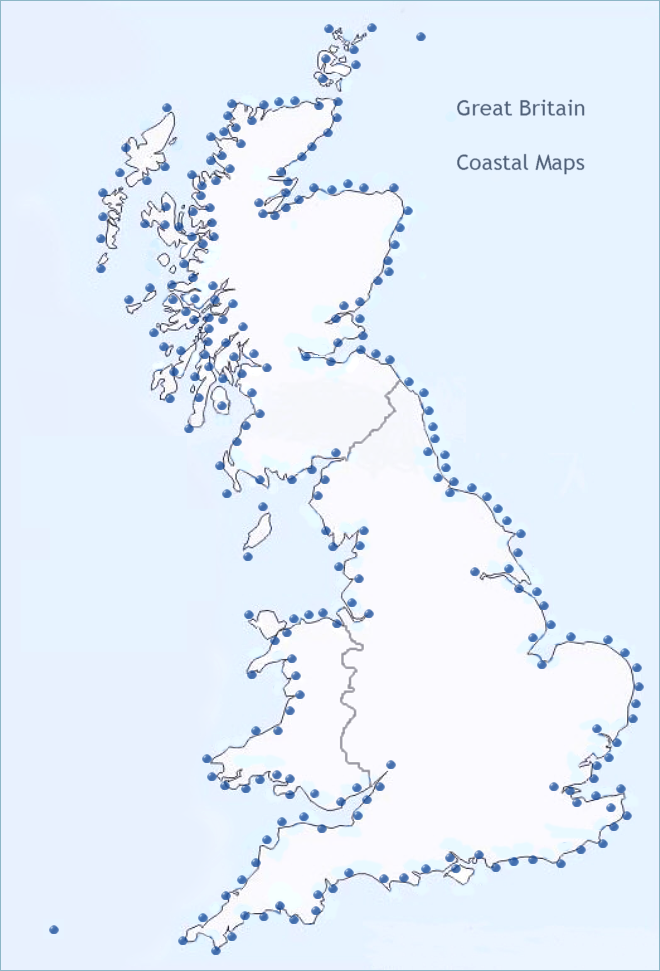
\includegraphics{britishcoastline.png}
}
\end{frame}

\begin{frame}{Background Definitions Pt 1}
	
	\begin{definition}[Hausdorff Measure]
	Let \(F\) be a subset of \(\mathbb{R}^{n}\) and \(s\geq 0\). For each \(\delta>0\), define
	\begin{align*}
		\mathcal{H}^{s}_{\delta}(F) = \inf \left\{\sum_{i=1}^{\infty} \left| U_i \right|^{s} \mid \left\{ U_i \right\} \text{ is a \(\delta\)-cover of \(F\)} \right\} .
	\end{align*}
The Hausdorff dimension looks at all covers of \(F\) of a certain dimension, and minimizes the \(s\)-th power of the diameters of the covering set. Notice that as \(\delta\) decreases, the class of permissible covers in \(F\) is reduced, and so the infimum increases. This gives us
\begin{align*}
	\mathcal{H}^{s}(F) = \lim_{\delta \to 0} \mathcal{H}^{s}_{\delta}(F)
\end{align*}
which we define the \textbf{\(s\)-dimensional Hausdorff measure of \(F\)}. This limit exists for any subset \(F\), but it can and will usually be \(0\) or \(\infty\).
\end{definition}

\end{frame}

\begin{frame}{Fractional Diameters?}
	\scalebox{0.5}{
	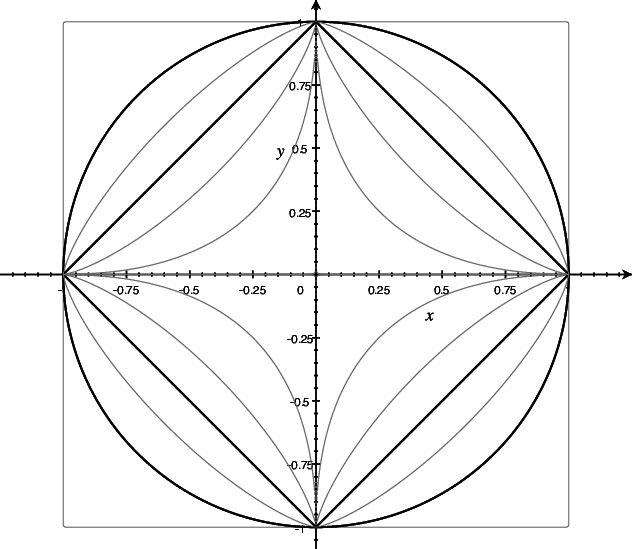
\includegraphics{fractionalcircle.png}}
\end{frame}

\begin{frame}{Britain coastline revisited}
	\scalebox{0.4}{
	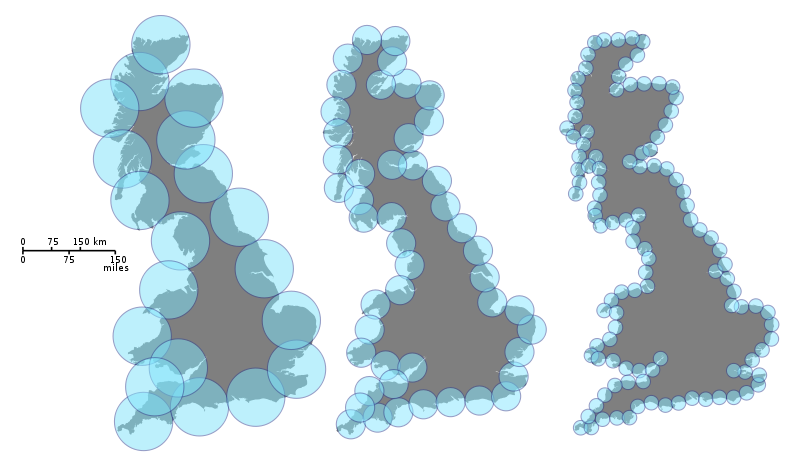
\includegraphics{Hausdorff.png}
}
\end{frame}



\begin{frame}{Background Definitions Pt 2}

	\begin{definition}[Hausdorff Dimension]
	Let \(F \subset \mathbb{R}^{n}\). Then the \textbf{Hausdorff dimension} of \(F\) is
	\begin{align*}
		\textrm{dim}_H F := \inf \left\{s \geq 0 \mid \mathcal{H}^{s}(F) = 0 \right\} = \sup \left\{s \mid \mathcal{H}^{s}(F) = \infty \right\} .
	\end{align*}
\end{definition}
This immediately gives
\begin{align*}
	\mathcal{H}^{s}(F) = \begin{cases}
		\infty & 0\leq s< \textrm{dim}_H F\\
		0 & s> \textrm{dim}_H F
	\end{cases}
\end{align*}
Note that for \(s =  \textrm{dim}_H F\), \(\mathcal{H}^{s}(F)\) can be zero, infinite, or finite. A Borel set that \(\mathcal{H}^{s}\) as finite is called an \(s\)-set.\\
\end{frame}


\begin{frame}
	\scalebox{0.4}{
	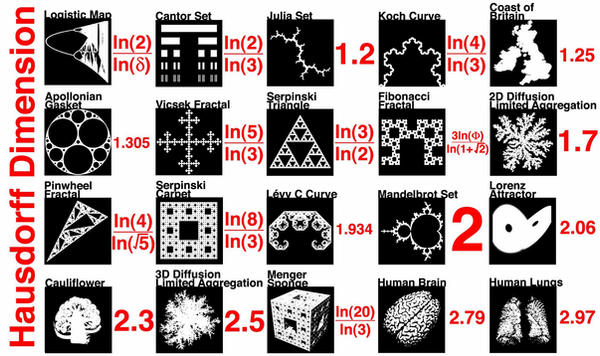
\includegraphics{hausdorffdimension.jpg}
}
\end{frame}

\begin{frame}{Background Definitions Pt 3}


\begin{definition}[Upper and lower densities]
	Let \(x \in \mathbb{R}^{n}\) and \(F\) be an \(s\)-set. The \textbf{lower} and \textbf{upper density} is given by
	\begin{align*}
		\underline{D}^{s}(F,x) = \underline{\textrm{lim}}_{r\to 0} \frac{\mathcal{H}^{s}(F\cap B(x,r))}{(2r)^{s}}\\
		\overline{D}^{s}(F,x) = \overline{\textrm{lim}}_{r\to 0} \frac{\mathcal{H}^{s}(F\cap B(x,r))}{(2r)^{s}}.
	\end{align*}
	If they both agree, then the density of \(F\) at \(x\) exists and is that value.
\end{definition}

\begin{definition}[Regular points]
	If \(\underline{D}^{s}(F,x) = \overline{D}^{s}(F,x) = 1\), then \(x\) is a \textbf{regular} point of \(F\), otherwise it is an \textbf{irregular} point.\\

	An \(s\)-set is called \textbf{regular} if, except on a set of \(\mathcal{H}^{s}\)-measure, all of its points are regular. If instead all of its points (except on a set of \(\mathcal{H}^{s}\) ) are irregular, then the \(s\)-set is \textbf{irregular}.
\end{definition}
\end{frame}

\begin{frame}{Examples of Regularity}
\begin{figure}[ht]
    \centering
     \def\svgwidth{1\linewidth}
     \input{./figures/square.pdf_tex}
    \caption{Square}
    \label{fig:square}
\end{figure}
\end{frame}

\begin{frame}{Examples of Irregularity}
\scalebox{0.2}{
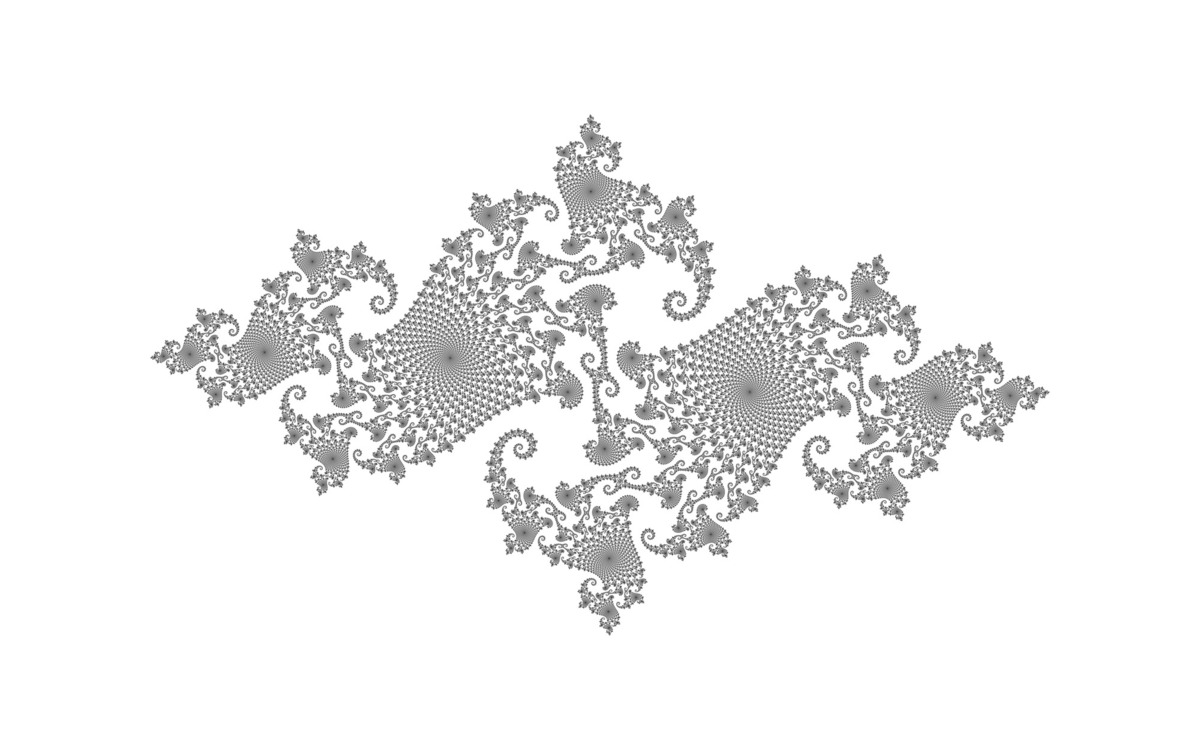
\includegraphics{irregularset.jpg}
}
\end{frame}

\begin{frame}[t]{Statement of Theorem}
	\begin{theorem}{Falconer 5.2}
	Let \(F\) be an \(s\)-set in \(\mathbb{R}^2\). Then \(F\) is irregular unless \(s\) is an integer.
\end{theorem}

	\scalebox{0.4}{
	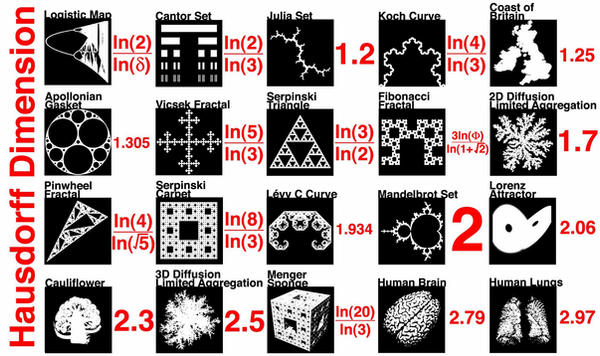
\includegraphics{hausdorffdimension.jpg}
}

\end{frame}

\begin{frame}[t]{Proof - Outline}
We will only show here the \(0<s<1\) case.

\begin{block}{Idea}
	Show that the density \(D^{s}(F,x)\) fails to exist almost everywhere in \(F\), by contradiction.
\end{block}
We assume for a contradiction that there is a set \(F_1\subset F\) of positive measure where \(\underline{D}^{s}(F,x) = \overline{D}^{s}(F,x)\).
% Implies by prop 5.1(b) that 1/2 < 2^-2 \leq D^s (F,x)

\vspace{15mm}

% Egoroff's Theorem:
% Let D be a Borel subset of Rn and mu a measure with mu(D) < inf. Let f1, f2, and f be functions from D to R such that f_k(x) -> f(x) for each x in D.

% Then Egoroff's theorem states that for any delta > 0, there is a Borel subset E of D such that mu(D \ E) < delta and the sequence {f_k} converges uniformly to f on E. In fact, we can choose E compact.

\begin{block}{Egoroff's Theorem}
	Tells us that there is \(r_0 > 0\), and Borel set \(E\subset F_1\) with \(\mathcal{H}^{s}(E) > 0\) such that
	\begin{align*}
		D^{s}(F,x) = \frac{\mathcal{H}^{s}(F\cap B(x,r))}{(2r)^{s}} > \frac{1}{2}
	\end{align*}
	for all \(x \in E\) and \(r<r_0\).
\end{block}
\end{frame}

\begin{frame}{Proof - Annulus}
	Let \(y \in E\) be a point with other points of \(E\) arbitrarily close. Let \(\eta \) satisfy \(0<\eta <1\), and consider the annulus given below:

\begin{figure}[ht]
\scalebox{0.75}{
    \centering
     \def\svgwidth{1\linewidth}
     \input{./figures/annulus.pdf_tex}
}
    \caption{Annulus}
    \label{fig:annulus}
\end{figure}
Observe that
\begin{align*}
	\lim_{r \to 0} \frac{\mathcal{H}^{s}(F\cap A_{r,\eta })}{(2r)^{s}} = D^{s}(F,y)((1+\eta )^{s}-(1-\eta )^{s})
\end{align*}

% We can choose a sequence of values r tending to 0 so that, we can choose x in E with |x-y| = r and B(x,r eta /2) cc A_r,eta
\end{frame}

\begin{frame}{Final Contradiction}
	Because \(y\) is a cluster point, there is always an \(x \in E\) with \(\left| x-y \right| =r\), and so by construction \(B(x,r \eta  / 2) \subset A_{r,\eta }\), yielding
	\begin{align*}
		\frac{\eta^{s}}{2} < \frac{\mathcal{H}^{s}(F\cap B(x,r \eta  / 2))}{r^{s}}\leq \mathcal{H}^{s}(F\cap A_{r,\eta })
	\end{align*}
	which combined with:
	\begin{align*}
		2^{-s-1}\eta^{s} \leq D^{s}(F,y)((1+\eta )^{s}-(1-\eta )^{s})\\
		= D^{s}(F,y)(2s \eta + \text{terms in }\eta^2)
	\end{align*}
	gives us a contradiction.
\end{frame}
% Take eta -> 0...

\begin{frame}{Credit}
	Huge thanks to Dr. Gregory Chambers for supporting and directing my work. Thanks to RUSP as well for contributing funding that enables our research.
\end{frame}

\begin{frame}{Questions?}
	
\end{frame}
\end{document}
